\chapter{Wo und Wie?}  % Kapitel % Steht dann über dem Text
\label{chapter:Wo und Wie?}  % Steht als Text im Inhaltsverzeichnis
\index{Wo und Wie?} % für das Stichwortverzeichnis

CodeRed kann jeder Nutzen der sich am System angemeldet hat. Wer welche Position oder Aufgaben im System übernimmt entscheiden die schon vorhandenen Mentoren. Ein User von Außerhalb kann sich zwar am System registrieren, ohne weiteren Kontakt zu einem Mentoren bleibt sein Account aber deaktiviert.\\
\\
Das Projekt CodeRed ist unter:\\
\centerline{\href{http://help.stsweilburg.de}{\textbf{http://help.stsweilburg.de}}\\ \href{https://help.stsweilburg.de}{\textbf{https://help.stsweilburg.de}}} \\
erreichbar.\\
\\ 
Zum Schutz ihrer Daten empfehlen wir den Zugang über die Sichere SSL\footnote[1]{Transport Layer Security (TLS) oder Secure Sockets Layer (SSL) ist ein Verschlüsselungsprotokoll für Datenübertragungen im Internet. TLS 1.0 und 1.1 sind die standardisierten Weiterentwicklungen von SSL 3.0.} Verbindung.
\newpage
\begin{figure}[h]
\begin{center}
   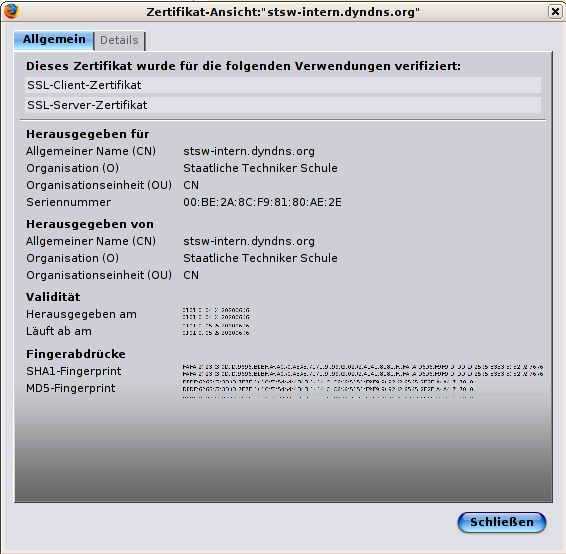
\includegraphics[width=370pt]{../bilder/certs2.png}
   \caption{Sichere SSL Verbindung}
   \label{Sichere SSL Verbindung}
\end{center}
\end{figure}
Für die Verschlüsselte Verbindung benutzt CodeRed ein Zertifikat mit einer 2048 Bit Verschlüsselung Da der Browser dieses Zertifikat nicht automatisch kennt, fragt der Browser den User ob das Zertifikat vertrauenswürdig ist. Um eine Verschlüsselte Verbindung aufzubauen muss hier das Zertifikat auf jedenfall angenommen werden. Ein Zertifikat das schon vom Browser als Sicher erkannt wird, kostet leider meist viel Geld. Für eine gesicherte Verbindung ist solch ein Zertifikat aber nicht nötig. 


